\subsection{Concurrent Streams on GPU}\label{sec:StreamGPU}
Heterogeneous computing is about efficiently using all processors in the system, including CPUs and GPUs.  In our heterogeneous systems, GPUs have been connected to a host machine by a high bandwidth interconnect such as PCI Express (PCIe). Host and device have different memory address spaces, and data must be copied back and forth between the two memory pools explicitly by the data transfer functions. 
%There are two main aspects to consider when attempting to run an application on both CPUs and GPUs concurrently, namely the communication costs incurred by CPU-GPU communications, and how to efficiently overlap computation and data transfers to reduce said cost.
%On integrated CPU/GPU architectures, ~\cite{Zhang17} suggested that the architecture differences between CPUs and GPUs, as well as limited shared memory bandwidth, are two main factors affecting co-running performance. 
%On SMP systems connected to GPU architectures, beside architectural differences, communications between CPUs and GPUs are another important factor. 
Servers with multi-cores and multi-accelerator devices are primarily connected by PCI-Express (PCIe) bus. GPUs and CPUs are bridged by a PCIe bus. Data are copied from the CPU host memory to PCIe memory first, and are then transferred to the GPU's global memory. The PCIe bandwidth is always a crucial performance bottleneck to be improved. 

Congestion control mechanisms have a significant impact on communications. Moreover, the PCIe congestion behavior varies significantly depending on the conflicts created by communication. \cite{Martinasso16} have explored the impact of PCIe topology, which is one major parameter influencing the available bandwidth. They developed a congestion-aware performance model for PCIe communication. They found that bandwidth distribution behavior is sensitive to the transfer message size. PCIe congestion can be hidden if the overlapping communications transfer very small message sizes. However, when the message size reaches some limit, congestion will significantly reduce the theoretical transfer bandwidth efficiency and the bandwidth between the CPU host memory and the GPU memory is far less than PCIe bandwidth. Nvidia provides ways to pin memory, also called paged-locked memory~\citep{CUDAGuide}. A pinned page can be remapped to a PCIe buffer to eliminate data transfer between the host memory and the PCIe buffer. However, consuming too much page-locked memory will reduces overall system performance.

CUDA's programming model provides constructs based on streaming which are capable to schedule multiple kernels concurrently. One CUDA stream can encapsulate multiple kernels, and they have to be scheduled so they strictly follow a particular order. However, kernels from multiple streams can be scheduled to run concurrently. Operations in different streams can be interleaved and overlapped, which can be used to hide data transfers between host and device.

A optimization of GPU applications is to overlap data transfers across the PCIe bus~\citep{Martinasso16}. This is only possible using CUDA streams and pinned memory in the host. Using pinned host memory enables asynchronous memory copies, lowers latency, and increases bandwidth. This way, streams can run concurrently. However, this goal is constrained by the number of kernel engines and copy engines exposed by GPUs, and synchronization must be explicit in the stream kernels. In order to obtain the best performance, a balance between computation and communication needs to be found. If the granularity is too fine, the performance can suffer from the increased communication overhead. On the other side, if the granularity is too coarse or bulk, the performance can suffer from load imbalance. 

There are GPUs with only a single copy engine and a single kernel engine. In this case, data transfer overlapping is not possible. Different streams may execute their commands concurrently or out of order with respect to each other. When an asynchronous CUDA stream is executed without specifying a stream, the CUDA runtime uses the default stream 0; but when a set of independent streams are executed with different ID numbers, these streams avoid serialization, achieving concurrency between kernels and data copies.

Figure~\ref{fig:streams} explains how the streaming model is used to improve the performance of GPU applications. In this figure, we compare the parallel CPU computations of two different GPU version with their respective data transfers: one single stream vs. 3 different kernels with their respective data transfers using 3 streams. The second method is only possible in GPUs with two copy engines, one for host-to-device transfers and another for device-to-host transfers. 


\begin{figure}
	\centering
%     \includegraphics[width=\linewidth]{fig/streams}
    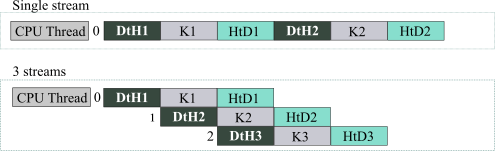
\includegraphics[scale=.8]{images/stream.png}
    \caption{Concurrent Streams overlapping data transfers}
    \label{fig:streams}
%\vspace{-15pt}
\end{figure}